\documentclass{article}
\pagestyle{headings}
\usepackage[utf8]{inputenc}
\usepackage[T1]{fontenc} 
\usepackage{eurosym}
\usepackage[english]{babel}
\usepackage{graphicx}
\usepackage{epsfig}
\usepackage{fancyhdr}
\usepackage{textcomp}
\usepackage{amssymb}
\usepackage{amsmath}
% \usepackage{relsize}    % decommenter (et installer le package) pour avoir un sous titre
\usepackage{amsthm}

\setlength{\textwidth}{370pt}
\lhead{}  % hides the left header (subsection name) which is overlapping with right header (section name)

\begin{document}

\newtheorem*{theorem}{Theorem}
\newtheorem*{definition}{Definition}
\newtheorem*{remark}{Remark}

\title{Titre}  % commenter cette ligne et décommentez la prochaine pour avoir un sous titre
%\title{Titre\\[0.07em]\smaller{}Sous titre}
\author{Votre nom}

\maketitle

\tableofcontents

\pagestyle{fancy}

\section{Introduction}
Blabla bla.\bigskip

blabla bla.\bigskip

blabla

\section{Les triangles}

\begin{definition}[Triangle rectangle]
Un triangle rectangle est ...
\end{definition}

blabla \bigskip

blablablabla

\begin{theorem}[Pythagore]
Le carré de l'hypothénuse est égal à la somme des carrés des longueurs des 2 côtés opposés.
\end{theorem}

cf \cite{tao} pour une preuve

\subsection{sous section}

blabla
\begin{itemize}
\item une ligne
\item une autre ligne avec une formule $f(x) = ax+b$
\end{itemize}

\begin{remark}
Attention à ne rien oublier.
\end{remark}

\begin{center}
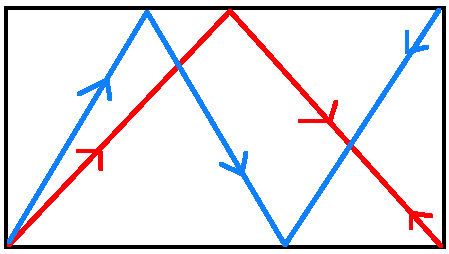
\includegraphics[width=3in,height=2.09in, clip]{images/billard.png}
\end{center}


\section{les cercles}

blabla 

\subsection{grands cercles}

\begin{definition}[cercle]
un cercle est un rond.
\end{definition}

\subsection{petits cercles}
blablabla
\begin{thebibliography}{9}
\bibitem{tao} 
T. Tao: Topics in random matrix theory
\\\texttt{https://terrytao.files.wordpress.com/2011/02/matrix-book.pdf}
\end{thebibliography}




\end{document}
